Dada las funciones de producción, la relación $RMS^A=RMS^B$ no es posible. En el gráfico se señala el nivel de producción que representa cada isocuanta, el cual depende de la cantidad de factores que se está utilizando. A modo de ejemplo, en el punto $\textbf{a}$ la empresa $A$ utiliza dos unidades de $K$ y ninguna de $L$ lo que llevado a su función de producción supone un output de dos unidades de $q_x$. La empresa $B$ en ese mismo punto utiliza dos unidades de $L$ y ninguna de $K$ ; sustituyendo en su función de producción se calcula un output de cuatro unidades de $q_y$. Las isocuantas que parten de a tienen anotado al lado esos valores de la producción. De modo similar se halla la producción que representan el resto de isocuantas.

\begin{center}
	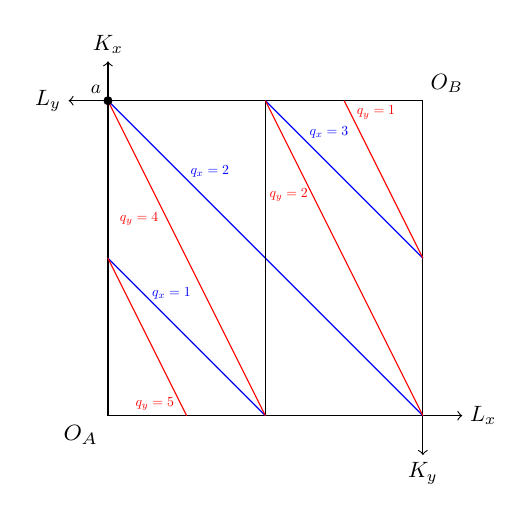
\begin{tikzpicture}
		% Caja
			\draw[<->] (0,4.5) node[align=center, above, scale=0.8] {$K_x$} -- (0,0) node[below left] {\footnotesize $O_A$} -- (4.5,0) node[align=center, right, scale=0.8] {$L_x$};
			\draw[<->] (-0.5,4) node[align=center, left, scale=0.8] {$L_y$} -- (4,4) node[align=center, above right, scale=0.8] {$O_B$} -- (4,-0.5) node[align=center, below, scale=0.8] {$K_y$};
		% Curvas de indiferencia
			% Para A
				\draw[blue] (0,2) -- (2,0);
				\draw[blue] (0,4) -- (4,0);
				\draw[blue] (2,4) -- (4,2);
			% Para B
				\draw (2,0) -- (2,4);
				\draw[red] (0,2) -- (1,0);
				\draw[red] (0,4) -- (2,0);
				\draw[red] (2,4) -- (4,0);
				\draw[red] (3,4) -- (4,2);
		% Etiquetas de producción
			% Para A
				\draw (0.5,1.55) node[right, scale=0.5, blue] {$q_x=1$};
				\draw (1.6,3.1) node[left, scale=0.5, blue] {$q_x=2$};
				\draw (2.5,3.6) node[right, scale=0.5, blue] {$q_x=3$};
			% Para B
				\draw (0.9,0.15) node[left, scale=0.5, red] {$q_y=5$};
				\draw (0.7,2.5) node[left, scale=0.5, red] {$q_y=4$};
				\draw (2.6,2.8) node[left, scale=0.5, red] {$q_y=2$};
				\draw (3.1,3.85) node[right, scale=0.5, red] {$q_y=1$};
		% Punto
			\draw[black, fill=black] (0,4) circle[radius=0.05] node [above left, scale=0.7] {$a$};
	\end{tikzpicture}
\end{center}

La eficiencia no se encuentra dentro de la caja debido a la forma de la función de producción; por ende, la solución es de esquina. La eficiencia se realiza en la asignación $\textbf{a}$ en donde se aprecia que un intercambio a lo largo de la isocuanta $q_x = 3$ o a lo largo de $q_y=2$ significa que una empresa mantiene su producción, pero a cambio de una merma en la producción de la otra. En consecuencia la asignación es eficiente.
\begin{center}
	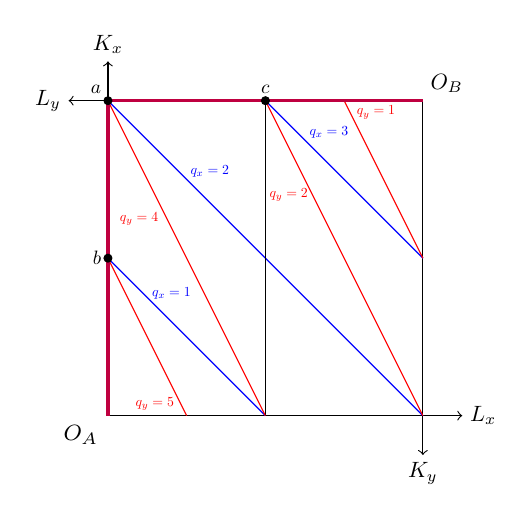
\begin{tikzpicture}
		% Caja
			\draw[<->] (0,4.5) node[align=center, above, scale=0.8] {$K_x$} -- (0,0) node[below left] {\footnotesize $O_A$} -- (4.5,0) node[align=center, right, scale=0.8] {$L_x$};
			\draw[<->] (-0.5,4) node[align=center, left, scale=0.8] {$L_y$} -- (4,4) node[align=center, above right, scale=0.8] {$O_B$} -- (4,-0.5) node[align=center, below, scale=0.8] {$K_y$};
		% Curvas de indiferencia
			% Para A
				\draw[blue] (0,2) -- (2,0);
				\draw[blue] (0,4) -- (4,0);
				\draw[blue] (2,4) -- (4,2);
			% Para B
				\draw (2,0) -- (2,4);
				\draw[red] (0,2) -- (1,0);
				\draw[red] (0,4) -- (2,0);
				\draw[red] (2,4) -- (4,0);
				\draw[red] (3,4) -- (4,2);
		% Etiquetas de producción
			% Para A
				\draw (0.5,1.55) node[right, scale=0.5, blue] {$q_x=1$};
				\draw (1.6,3.1) node[left, scale=0.5, blue] {$q_x=2$};
				\draw (2.5,3.6) node[right, scale=0.5, blue] {$q_x=3$};
			% Para B
				\draw (0.9,0.15) node[left, scale=0.5, red] {$q_y=5$};
				\draw (0.7,2.5) node[left, scale=0.5, red] {$q_y=4$};
				\draw (2.6,2.8) node[left, scale=0.5, red] {$q_y=2$};
				\draw (3.1,3.85) node[right, scale=0.5, red] {$q_y=1$};
		% Curva de contrato
			\draw[purple, very thick] (0,0) -- (0,4) -- (4,4);
		% Punto
			\draw[black, fill=black] (0,2) circle[radius=0.05] node [left, scale=0.7] {$b$};
			\draw[black, fill=black] (0,4) circle[radius=0.05] node [above left, scale=0.7] {$a$};
			\draw[black, fill=black] (2,4) circle[radius=0.05] node [above, scale=0.7] {$c$};
	\end{tikzpicture}
\end{center}

Para graficar la FPP, se ubican los puntos respectivos. Si la empresa $A$ utiliza todo los factores de producción entonces $q_x = 2 + 2 = 4$, mientras que que la empresa $B$ no produce nada $q_y = 2\times 0 + 0 = 0$ siendo $(q_x, q_y)=(4,0)$ un par ordenado en la FPP. Análogamente para la empresa $B$ sería $q_y = 2\times2 + 2 = 6$ y para $A$ un $q_x=0$ siendo $(q_x, q_y)=(0,6)$ otro par ordenado. Del mismo modo en la puntos $a, b$ y $c$ se obtienen los pares ordenados $(2,4), 1,5)$ y $(3,2)$.

\begin{center}
	\begin{tikzpicture}
		% Ejes
			\draw[<->] (0,6.5) node[align=center, above, scale=0.8] {$q_y$} -- (0,0) -- (4.5,0) node[align=center, right, scale=0.8] {$q_x$};
	
		% FPP
			\draw[purple] (0,6) node[left, scale=0.8, black] {$6$} -- (1,5) -- (2,4) -- (3,2) -- (4,0) node[below, scale=0.8, black] {$4$};
	
		% Líneas punteadas
			\draw[dashed] (1,0) node[below, scale=0.8] {$1$} -- (1,5) node[above right, scale=0.8] {$b$} -- (0,5) node[left, scale=0.8] {$5$};
			\draw[dashed] (2,0) node[below, scale=0.8] {$2$} -- (2,4) node[above right, scale=0.8] {$a$} -- (0,4) node[left, scale=0.8] {$4$};
			\draw[dashed] (3,0) node[below, scale=0.8] {$3$} -- (3,2) node[above right, scale=0.8] {$c$} -- (0,2) node[left, scale=0.8] {$2$};
		% Puntos
			\draw[black, fill=black] (1,5) circle[radius=0.05];
			\draw[black, fill=black] (2,4) circle[radius=0.05];
			\draw[black, fill=black] (3,2) circle[radius=0.05];
	\end{tikzpicture}
\end{center}